% Drawing 144/06-3 -- folder 144, batch 06, archive page 104 (PDF page 105).
% Transcription: Deux sphères. Sur la première, un cercle horizontal portant $-1$, $0$, $1$, $\infty$ ; lacets fléchés $\lambda'_{1/2}$, $\lambda'_1$, $\lambda'_\infty$ autour des points, et un chemin marqué $3$. Sur la seconde, le pôle marqué $-\bar{j}$, un méridien épais descendant au point $1/2$ du cercle équatorial (en tirets), les points $0$, $1$, $\infty$ ; une petite flèche tourne autour de $1/2$. À droite, un fuseau (lentille) coupé par deux segments perpendiculaires.
% Kind: two spheres with loops and a meridian; a lens cut by two segments. Method 2 (schematic redraw from the facsimile). Status: partial.
% Notes: Each figure re-read on its own tight crop; points computed on the circles they lie on, and loops and meridians drawn to them. First sphere: the outline, the horizontal circle (solid in front, dashed at the left), the points -1, 0, 1, infinity on it, a small loop round 0, a closed loop round 1, the arrowed loop lambda'_infty round infinity, the short arrow marked 3 and a long dashed arrowed path from the top towards 1; labels lambda'_{1/2}, lambda'_1, lambda'_infty where he wrote them. Second sphere: the outline, the pole -j bar, the thick meridian from the pole down to 1/2 on the equator and dashed below it, the dashed meridian from the pole to infinity at the back, a thin arc from the pole down the left, the equator dashed at the back and solid in front through 0, 1/2, 1, a small loop round 0 and the small arrow turning round 1/2. Right: the lens cut by a horizontal and a vertical segment meeting at its centre. Labels \small. Still differs from the facsimile: the first sphere is a rough sketch on the page, with an irregular outline and several strokes whose course is unclear (the long path, the arc at its right); the loops lambda'_{1/2} and lambda'_1 are labelled but their strokes are not separated from the others; on the lens, the horizontal segment is broken on each side of the centre on the page and drawn whole. The formula "2z - 1" and the arrow lambda_{1/2} above the lens are text. Redrawn 2026-11-09 (issue 128): to check again. Overlay check 2026-11-13 (issue 147, Claude Opus 5.5): the redraw, rasterised from its TikZ paths, laid over the 300 dpi colour render of the 250 ppi scan with the contrast raised. The second sphere (outline, pole, meridians, equator, points and the small arrow) and the lens lie on their ink to within about 1 unit; the thin arc from the pole down the left of the second sphere and the upper arc of the lens are faint and only partly inked. Nothing changed. Still differs then: on the first sphere the outline was an ellipse up to 2 units off the page (redrawn on 2026-11-14, below), and the loops lambda'_{1/2} and lambda'_1 and the long dashed path cannot be told apart from the other strokes there, as said above; the horizontal segment of the lens is broken on the page and drawn whole. Not compiled (no TeX engine in the session). 2026-11-14, Claude Opus 5.5, issue 147 second pass: on the first sphere, the outline redrawn stroke by stroke through points read on a gridded crop of the 400 dpi scan at 34 pixels per unit: an open curve, as on the page, from its lower end under 0 round the left, the flattened top and the wide right side down to its end under the loop round 1; the horizontal circle redrawn the same way (the heavy top from the start of the arrow 3 through infinity, the dashed left part round -1 down to 0, the heavy bottom from 0 to its blot at 1, and the pencil continuation right of infinity, which stops short of the right rim), with the four points on their blots; the loops round 0 and round 1, the loop lambda'_infty and the arrow 3 moved onto their ink; the inner arc at the right (from the top of the rim down towards the horizontal circle) added. Overlay with the local TikZ interpreter (not compiled: no TeX in the session): these lie on their ink to within about half a unit. Still differs: the strokes of the loops lambda'_{1/2} and lambda'_1 are still not told apart from the long dashed path and the short strokes near them, and the horizontal segment of the lens is broken on the page and drawn whole.
% Coordinates: 1 unit = 1 mm = 1/100 of the crop width (bbox in page fractions: [0.18, 0.27, 0.89, 0.42]).
% Redrawn by Claude (claude-opus-5-5), issue #73, 2026-11-09; not checked by a human; not compiled (no TeX in the session).
% Checked by Claude (claude-opus-5-5) 2026-11-13 (issue #147): overlay on the 300 dpi colour render of the 250 ppi scan; nothing changed; not compiled (no TeX in the session). Not checked by a human. Status: partial.
% Rights: reproduces part of the work -- behind RENDER_TRANSCRIPTS, never published by itself.
\documentclass[tikz,border=3pt]{standalone}
\usepackage{amsmath,amssymb}
\usetikzlibrary{patterns,arrows.meta}
\tikzset{pencil/.style={black!45}, struck/.style={black!35}, mark/.style={circle,draw,inner sep=1.3pt}, pt/.style={circle,fill,inner sep=0.9pt}, opt/.style={circle,draw,fill=white,inner sep=1.1pt}}
\begin{document}
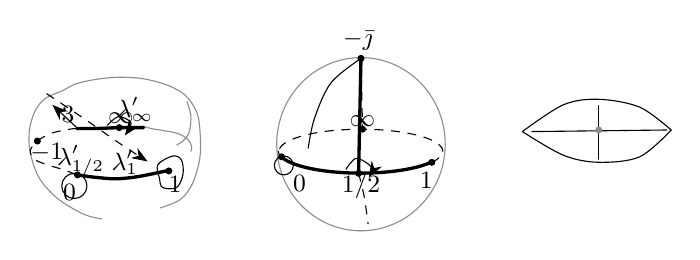
\begin{tikzpicture}[x=1mm,y=1mm,line cap=round,line join=round,font=\scriptsize]
\draw[pencil] plot[smooth, tension=0.55] coordinates {(12.9,-25.6) (10.6,-25) (7.4,-23.1) (5,-20.5) (3.8,-17.2) (3.7,-14.3) (4.4,-11.9) (5.7,-10.3) (7.9,-9.3) (9.7,-8.4) (12.6,-7.8) (15.3,-7.6) (18.2,-7.8) (21.2,-8.6) (23.5,-9.9) (25,-12.2) (25.4,-15.2) (25.3,-18.1) (24.4,-21.1) (22.9,-23.1) (20.3,-24.2)};
\draw[pencil] plot[smooth, tension=0.55] coordinates {(18.2,-13.8) (19.1,-14.1) (22.4,-14.7) (23.8,-15.5) (24.3,-16.4) (24.2,-17)};
\draw[pencil] plot[smooth, tension=0.55] coordinates {(23.7,-10.7) (24.2,-12.5) (24,-14.5) (23.3,-15.6) (22.4,-16.2)};
\draw[very thick] plot[smooth, tension=0.5] coordinates {(9.7,-14.1) (12.4,-14.1) (15.1,-14) (18.2,-14)};
\draw[dashed] plot[smooth, tension=0.5] coordinates {(9.7,-14.1) (8.8,-14.2) (6.5,-14.7) (4.7,-15.7) (3.8,-16.9) (4.3,-18) (5.9,-18.7) (8.2,-19.4) (9.7,-20)};
\draw[very thick] plot[smooth, tension=0.5] coordinates {(9.7,-20) (12,-20.3) (14.7,-20.5) (17.6,-20.2) (21.5,-19.4)};
\node[pt] at (9.8,-20) {};
\node[pt] at (21.4,-19.5) {};
\node[pt] at (4.7,-15.7) {};
\node[pt] at (15.1,-14) {};
\draw (9.4,-21.4) circle[radius=1.6];
\draw plot[smooth cycle, tension=0.55] coordinates {(20,-18.7) (21.9,-17.6) (23,-18.1) (23.2,-19.9) (22.4,-21.6) (20.6,-21.6) (20.2,-20.4)};
\draw[-{Stealth[length=2mm]}] plot[smooth, tension=0.55] coordinates {(13.6,-13.7) (15,-12.6) (16.6,-13.4) (15.8,-15)};
\draw[-{Stealth[length=2mm]}] (9.6,-13.9) -- (6.6,-11.1);
\draw[dashed,-{Stealth[length=2mm]}] plot[smooth, tension=0.55] coordinates {(5.9,-9.7) (10.7,-12.9) (15,-15.9) (18.7,-18.3)};
\node[inner sep=1pt] at (8.8,-22.2) {\small $0$};
\node[inner sep=1pt] at (22.2,-21.2) {\small $1$};
\node[inner sep=1pt] at (5.9,-17.2) {\small $-1$};
\node[inner sep=1pt] at (15.3,-12.8) {\small $\infty$};
\node[inner sep=1pt] at (8.6,-12.3) {\small $3$};
\node[inner sep=1pt] at (17.1,-11.7) {\small $\lambda'_\infty$};
\node[inner sep=1pt] at (10.2,-18.2) {\small $\lambda'_{1/2}$};
\node[inner sep=1pt] at (15.8,-18.4) {\small $\lambda'_1$};
\draw[pencil] (45.8,-16.1) ellipse[x radius=10.7, y radius=11];
\draw[dashed] (56.2,-17) arc[start angle=0, end angle=180, x radius=10.4, y radius=2.8];
\draw[dashed] (35.3,-17) arc[start angle=180, end angle=195, x radius=10.4, y radius=2.8];
\draw[very thick] (35.7,-17.7) arc[start angle=195, end angle=330, x radius=10.4, y radius=2.8];
\draw[dashed] (54.8,-18.4) arc[start angle=330, end angle=360, x radius=10.4, y radius=2.8];
\draw[very thick] (45.8,-5.2) -- (45.5,-19.8);
\draw[dashed] (45.8,-5.2) -- (46,-14.2);
\draw[dashed] plot[smooth, tension=0.55] coordinates {(45.5,-19.8) (46.2,-22.7) (46.7,-26.2)};
\draw plot[smooth, tension=0.55] coordinates {(45.8,-5.2) (42,-8.3) (39.9,-12.8) (39.1,-16.6)};
\draw (36,-18.8) circle[radius=1.2];
\draw[-{Stealth[length=2mm]}] plot[smooth, tension=0.55] coordinates {(43.9,-19.3) (45.2,-17.9) (47.1,-19) (46.8,-20.3)};
\node[pt] at (45.8,-5.2) {};
\node[pt] at (35.7,-17.7) {};
\node[pt] at (45.5,-19.8) {};
\node[pt] at (54.8,-18.4) {};
\node[pt] at (46,-14.2) {};
\node[inner sep=1pt] at (45.4,-2.9) {\small $-\bar{\jmath}$};
\node[inner sep=1pt] at (46,-13.2) {\small $\infty$};
\node[inner sep=1pt] at (38,-21.1) {\small $0$};
\node[inner sep=1pt] at (45.8,-21.5) {\small $1/2$};
\node[inner sep=1pt] at (54.1,-20.7) {\small $1$};
\draw plot[smooth, tension=0.55] coordinates {(66.3,-14.5) (71.5,-11.1) (76,-10.4) (81.2,-11.4) (85.2,-14.3)};
\draw plot[smooth, tension=0.55] coordinates {(66.3,-14.5) (71.5,-17.5) (76,-18.4) (81.2,-17.7) (85.2,-14.3)};
\draw (67.5,-14.5) -- (84.6,-14.3);
\draw (76,-11.2) -- (76,-18);
\node[pt,pencil] at (76,-14.3) {};
\end{tikzpicture}
\end{document}
